\documentclass[a4paper]{ctexart}
\usepackage[top=2.3cm,bottom=2cm,left=1.7cm,right=1.7cm]{geometry} 
\usepackage{amsmath, amssymb}
\usepackage{mathrsfs} 
\usepackage{booktabs}
\usepackage{amsthm}
\usepackage{longtable} 
\usepackage{graphicx}
\usepackage{subfigure}
\usepackage{caption}
\usepackage{fontspec}
\usepackage{titlesec}
\usepackage{fancyhdr}
\usepackage{latexsym}
\def\d{\mathrm{d}}
\def\e{\mathrm{e}}
\def\degree{$^{\circ}$}
\title{\textbf{中心力场问题\&小振动}}
\author{王崇斌 1800011716}
\date{}
\makeatletter %使\section中的内容左对齐
\renewcommand{\section}{\@startsection{section}{1}{0mm}
	{-\baselineskip}{0.5\baselineskip}{\bf\leftline}}
\makeatother
\begin{document}
    \pagestyle{fancy}
    \lhead{理论力学作业}
	\chead{}
	\rhead{}
	\maketitle
    \thispagestyle{fancy}
    \paragraph{第一题}
    人们通常把航天器达到环绕地球、脱离地球和飞出太阳系所需要的最小发射速度,分别称为
    第一宇宙速度、第二宇宙速度(也称脱离速度)和第三宇宙速度(也称太阳的逃逸速度)
    \subparagraph{(a)}\;在地球赤道处以第一宇宙速度的一半和仰角45\degree 发射一个物体,求物体
    以OA为极轴的轨道方程。
    \subparagraph{解}:
    考虑第一宇宙速度的计算,可以看出这个速度是将地球当作球体,使得飞船贴地匀速圆周运动的速度,
    可以根据万有引力和向心力公式给出,其中$M$是地球质量,$m$是发射物体的质量,$R$为地球的平均
    半径,$G$为万有引力常数:
    \begin{align}
        \frac{GMm}{R^{2}} = m \frac{v_{1}^{2}}{R}
    \end{align}
    化简后可得$v_{1}$表达式:
    \begin{align}
        v_{1} = \sqrt{\frac{GM}{R}}
    \end{align}
    根据题目中的数据可以给出此问题两个运动积分能量$E$与角动量$J$的数值:
    \begin{align}
        E &= \frac{1}{2}mv^{2} - \frac{GMm}{R} = -\frac{7}{8}\frac{GMm}{R}\\
        J &= mv_{\theta}R = \frac{m}{4}\sqrt{2GMR}
    \end{align}
    选取物体距离地心O的距离$r$与物体距离地心的位矢与OA轴的夹角$\theta$为广义坐标,
    考虑地球静止不动,我们直接给出能量的表达式:
    \begin{align}
        E & = \frac{1}{2}mv^{2} + U(r)\\
          & = \frac{1}{2}m(\dot{r}^{2} + r^{2}\dot{\theta}^{2}) - \frac{GMm}{r}\\
          & = \frac{1}{2}m\dot{r}^{2} + \frac{J^{2}}{2mr^{2}} - \frac{GMm}{r}
    \end{align}
    可以得到:
    \begin{align}
        \frac{\d r}{\d t} &= \sqrt{2\left(\frac{E}{m} + \frac{GM}{r}\right) - \frac{J^{2}}{mr^{2}}}\\
        \frac{\d \theta}{\d t} &= \frac{J}{mr^{2}}
    \end{align}
    可以得到轨道的微分方程为:
    \begin{align}
        \frac{\d \theta}{\d r} = \frac{J / r^{2}}{\sqrt{2\left(E + \frac{GMm}{r}\right) - \frac{J^{2}}{r^{2}}}}
    \end{align}
    积分后可得:
    \begin{align}
        \frac{p}{r} &= e\cos(\theta + \theta_{0}) + 1\\
        p &= \frac{J^{2}}{GMm^{2}}\\
        e &= \sqrt{1 + \frac{2EJ^{2}}{G^{2}M^{2}m^{3}}}
    \end{align}
    其中$\theta_{0}$是一个常数,需要初始条件来确定,带入初始条件后可得:
    \begin{align}
        \frac{R}{8r} = \frac{5\sqrt{2}}{8}\cos(\theta + 3.00) + 1
    \end{align}
    其中角度的单位为弧度(早知道这题就直接代公式了)
    \subparagraph{(b)}
    把地球和金星绕太阳的运动近似看成在共面的圆,半径分别为$R_{0}$与$0.7R_{0}$,现从地面发射一个
    如图中所示的轨道的人造卫星去考察金星,发射的最小速度为多少?
    \subparagraph{解:}
    我们首先计算在只考虑太阳引力(不计地球和金星的引力影响)的情况下,在这样一个轨道上运行需要的一些限制条件。
    设太阳质量为$M_{0}$,人造卫星质量为$m$,近日点距离为$r_{1}$,远日点距离为$r_{2}$。考虑到轨道方程,可得:
    \begin{align}
        r_{1} &= \frac{p}{1 + e}\\
        r_{2} &= \frac{p}{1 - e}\\
        p &= \frac{J^{2}}{GM_{0}m^{2}}
    \end{align}
    解出$J$的表达式:
    \begin{align}
        J = m\sqrt{\frac{2GM_{0}r_{1}r_{2}}{r_{1} + r_{2}}}
    \end{align}
    可以算出卫星到达远日点时的速度为:
    \begin{align}
        v = \frac{J}{mr_{2}} = \sqrt{\frac{2GM_{0}r_{1}}{r_{2}(r_{1} + r_{2})}}
    \end{align}
    上面算出的速度实际上是卫星已经完全脱离地球引力时的速度,并不是从地面发射的速度。考虑地球上发射卫星的
    速度为$v_{0}$,它通过一系列运动脱离地球引力的影响,假设在这个过程中卫星与太阳的距离变化很小,忽略太阳
    的引力影响,脱离地球引力后,其在地球参考系的速度为$v'$。为了使$v_{0}$最小,我们考虑$v'$与地球相对
    太阳的速度$\Delta v$方向相同,只要这两个速度之和等于$v$即可。那么我们有:
    \begin{align}
        v &= v' + \Delta v\\
        \frac{GMm}{R} &= \frac{1}{2}mv_{0}^{2} - \frac{1}{2}mv'^{2}\\
        \Delta v &= \sqrt{\frac{GM_{0}}{R_{0}}}
    \end{align}
    带入数据计算得:
    \begin{align}
        v = \sqrt{\frac{1.4GM}{1.7R_{0}}}
    \end{align}
    可以看到这个速度要比地球绕太阳运动的速度小,即如果按第二宇宙速度发射,会使得卫星在太阳系中的速度大于我们预设
    的速度,但是如果发射速度小于第二宇宙速度,会使得卫星无法脱离地球引力(这个过程中还是忽略了太阳的影响,不然没法算了),
    因此我认为最小的发射速度就是第二宇宙速度,应该在飞离地球引力范围后再考虑减速,使之回到预设的轨道。(虽然我觉得
    这很奇怪,但是目前也就能想到这么多了)
    \subparagraph{(c)}
    题目略
    \subparagraph{解:}首先得讨论一下第三宇宙速度是多大。卫星先脱离地球引力,会剩余一个相对于地球的速度
    这个速度加上地球的公转速度(最小情况,是两个速度共线直接相加),就是卫星在太阳系中的速度,只要
    此时卫星可以摆脱太阳引力即可。所有的物理量的记号均与之前相同。挣脱地球引力后在太阳系中的速度$v$由下式
    确定:
    \begin{align}
        \frac{1}{2}mv^{2} - \frac{GM_{0}m}{R_{0}} = 0
    \end{align}
    可得卫星挣脱地球引力后在地球系的最小速度$v'$为:
    \begin{align}
        v' = (\sqrt{2} - 1)\sqrt{\frac{GM_{0}}{R_{0}}}
    \end{align}
    那么可得$v_{3}$的表达式:
    \begin{align}
        v_{3} = \sqrt{\frac{2GM}{R} + (3-2\sqrt{2})\frac{GM_{0}}{R_{0}}}
    \end{align}
    那么我们可以算出当卫星以第三宇宙速度发射后摆脱地球引力时速度的大小:
    \begin{align}
        v' = (\sqrt{2} - 1)\sqrt{\frac{GM_{0}}{R_{0}}}
    \end{align}
    由于认为地球轨道是圆形,那么地球相对太阳的速度与飞船相对于地球的速度垂直,很容易将飞船
    相对于太阳的速度分解为径向速度和角向速度:
    \begin{align}
        v_{r} &= v' = (\sqrt{2} - 1)\sqrt{\frac{GM_{0}}{R_{0}}}\\
        v_{\theta} &= \sqrt{\frac{GM_{0}}{R_{0}}}
    \end{align}
    那么可以计算出角动量与能量:
    \begin{align}
        J &= mv_{\theta}R_{0} = m\sqrt{GM_{0}R_{0}}\\
        E &= \frac{1}{2}m(v_{r}^{2} + v_{\theta}^{2}) - \frac{GM_{0}m}{R_{0}}=(1 - \sqrt{2})\frac{GM_{0}}{R_{0}} 
    \end{align}
    带入轨道方程的表达式可得轨道方程为:
    \begin{align}
        \frac{R_{0}}{r} = (\sqrt{2} - 1)\cos(\theta) + 1
    \end{align}
    其中选择椭圆的长轴处$\theta = 0$。
    \\
    \paragraph{第二题\;\;中心力场中的圆轨道}题目略
    \subparagraph{(a)}两体问题的约化
    \subparagraph{解:}
    首先考虑使用两个粒子各自的坐标为广义坐标,可以得到系统的拉格朗日量:
    \begin{align}
        L = T - V = \frac{1}{2}m_{1}(\dot{\vec{x_{1}}})^{2} + \frac{1}{2}m_{2}(\dot{\vec{x_{2}}})^{2} - k|\vec{x_{1}} - \vec{x_{2}}|^{\beta}
    \end{align}
    考虑质心的定义:
    \begin{align}
        \vec{R} = \frac{m_{1}\vec{x_{1}} + m_{2}\vec{x_{2}}}{m_{1} + m_{2}}
    \end{align}
    可以解出:
    \begin{align}
        \vec{x_{1}} &= \vec{R} + \frac{m_{2}}{m_{1} + m_{2}}\vec{x}\\
        \vec{x_{2}} &= \vec{R} - \frac{m_{1}}{m_{1} + m_{2}}\vec{x}
    \end{align}
    带入之前拉格朗日量的表达式,同时考虑到质心速度为常数可以忽略,同时忽略速度的全导项,那么拉格朗日
    量可以化简为:
    \begin{align}
        L = \frac{1}{2}\frac{m_{1}m_{2}}{m_{1} + m_{2}}(\dot{\vec{x}})^{2} - kx^{\beta}
    \end{align}
    将质心选为坐标原点,即$\vec{R}=0$,那么容易将拉格朗日量化简为上述形式。如果我们定义一个粒子的质量为
    $m = \frac{m_{1}m_{2}}{m_{1} + m_{2}}$,那么上述拉格朗日量可以看作此粒子单独在外场中运动的方程,
    即将两体问题化简为了单体问题。对于这个系统,由拉格朗日量不显含时间可知能量守恒;由绕势场中心的转动不变性
    可知角动量守恒,进一步得知粒子的运动应被限制在一个平面内,那么我们可以选择极坐标作为广义坐标,拉格朗日量
    可写为:
    \begin{align}
        L = \frac{1}{2}m(\dot{r}^{2} + r^{2}\dot{\theta}^{2}) - kr^{\beta}
    \end{align}
    系统的角动量可表达为:
    \begin{align}
        J = \frac{\partial L}{\partial \dot{\theta}} = mr^{2}\dot{\theta}
    \end{align}
    带入能量的表达式:
    \begin{align}
        E = \frac{1}{2}m\dot{r}^{2} + \frac{J^{2}}{2mr^{2}} + kr^{\beta}
    \end{align}
    上面的表达式完全可以看作粒子在一个势场中做一维运动的情形,此时有效势能为:
    \begin{align}
        U_{eff} = \frac{J^{2}}{2mr^{2}} + kr^{\beta}
    \end{align}
    (在解答时注意到了一个问题,本来是想着把运动积分带入拉格朗日量后讨论运动方程,、
    但是这样做有明显的问题,是不是因为拉格朗日量只有写作广义坐标的函数时才有讨论
    运动方程的意义?那么为什么用能量可以方便地类比,是因为可以直接给出一个类似于
    一维运动的微分方程的原因么)
    \subparagraph{(b)}圆轨道的稳定性
    \subparagraph{解:}
    圆轨道保证了径向坐标为常数,那么这时一定是$\frac{\partial U_{eff}}{\partial r} = 0$的
    位置,否则粒子会受到一个等效的径向力让它偏离$r$的位置,不再是按照圆轨道运动。如果给此时的
    轨道一个扰动,一般情况下粒子会偏离有效势能曲线的稳定点;如果此稳定点是极小值点(二阶导数大于零),那么只要在
    极小值点足够小的邻域内,无论系统偏离向$r$增大或减小的方向,都会受到一个等效的作用力使得系统回到平衡位置(分析
    有效势能在极小值点邻域内的导数就行);同理,如果稳定点是有效势能曲线的极大值点,无论向$r$增大或减小的方向偏离,
    都会使得系统受到远离平衡位置的作用力;如果稳定点不是极值点,那么必然有一个方向的偏离会使得系统收到远离平衡位置的
    作用力。因此只有粒子处于有效势能曲线的极小值点时,圆轨道才是稳定平衡位置,或者说只有当有效势能曲线有极小值点时,
    粒子在圆轨道上的运动才是稳定的。可得对于有效势能的约束条件:
    \begin{align}
        \frac{\d U_{eff}}{\d r}(r_{0}) &= 0\\
        \frac{\d ^{2} U_{eff}}{\d r^{2}} &> 0
    \end{align}
    带入上一问$U_{eff}$的表达式,化简上式,并注意到$k$与$\beta$同号,可得到:
    \begin{align}
        \beta > -2
    \end{align}
    \subparagraph{(c)}圆轨道时的径向微扰
    \subparagraph{解:}题目中$r(t) = r_{0} + \eta(t)$的微扰形式已经说明了这是一个径向微扰,那么不会改变系统原有的
    角动量,也可以近似地认为系统的能量并不发生变化,分别写出微扰前与微扰后的能量守恒表达式:
    \begin{align}
        E & = \frac{J^{2}}{2mr^{2}_{0}} + kr_{0}^{\beta}\\
        E &= \frac{1}{2}m\dot{r}(t)^{2} + \frac{J^{2}}{2mr(t)^{2}} + kr(t)^{\beta}
    \end{align}
    考虑到微扰很小,我们把微扰后的能量表达式Taylor展开,注意要展开到二阶,同时带入微扰前的能量表达式和圆轨道的约束条件:
    \begin{align}
        0 = m\dot{\eta}^{2} + k\beta r_{0}^{\beta - 2}(2 + \beta)\eta^{2}
    \end{align}
    上式两边求导后可得一标准的简谐振动方程:
    \begin{align}
        \ddot{\eta} + \frac{k\beta r_{0}^{\beta - 2}(2 + \beta)}{m}\eta = 0
    \end{align}
    容易看出其简谐振动的频率为:$\delta\omega = \sqrt{\frac{k\beta r_{0}^{\beta - 2}(2 + \beta)}{m}}$
    \subparagraph{(d)}微扰下轨道的闭合性
    \subparagraph{解:}
    首先计算圆轨道的圆频率:
    \begin{align}
        k\beta r^{\beta - 1} = m \omega^{2}r\\
        \omega = \sqrt{\frac{k\beta r^{\beta - 2}}{m}}
    \end{align}
    带入题中数据$\beta = \frac{15}{25},\;-\frac{2}{9}$
    \begin{align}
        \frac{\delta\omega}{\omega_{1}} &= \frac{\sqrt{65}}{5}\\
        \frac{\delta\omega}{\omega_{2}} &= \frac{4}{3}
    \end{align}
    可以看出第一个比值不为有理数,故不能形成闭合的轨道,第二种情况由于角频率比值为有理数,
    可以形成闭合的轨道。
    \begin{figure}[ht]
        \centering
        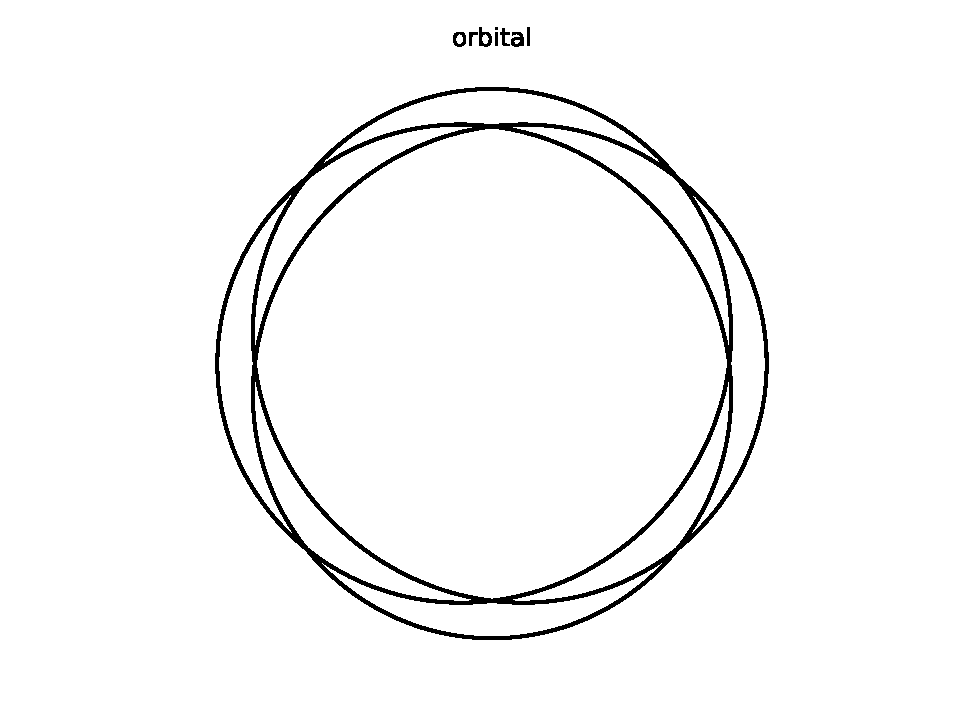
\includegraphics[scale=0.46]{orbital.pdf}
        \caption{粒子受到微扰之后的运动轨道}
    \end{figure}
    \paragraph{第三题\;\;散射问题}
    \subparagraph{解:}考虑偏转角$\Theta$与瞄准距离$s$之间的关系:
    \begin{align}
        \Theta(s) &= \pi - 2\phi(s)\\
        \phi(s) &= \int_{r_{0}}^{+\infty}\frac{J/r^{2}\d r}{\sqrt{2m[E - V(r)] - J^{2}/r^{2}}}
    \end{align}
    其中$r_{0}$为距离散射中心的最小距离,带入$E$与$J$的表达式:
    \begin{align}
        E = \frac{1}{2}mv_{0}^{2}\\
        J = mv_{0}s
    \end{align}
    其中$v_{0}$为无穷远处速度,带入并化简:
    \begin{align}
        \Theta(s) &= \pi - 2s\int_{r_{0}}^{+\infty}\frac{\d r}{r\sqrt{r^{2}[1 - V(r)/E] - s^{2}}}
    \end{align}
    作变换$u = \frac{r_{0}}{r}$,可以将积分化为:
    \begin{align}
        \Theta(s) = \pi - 2s\int_{0}^{1}\frac{\d u}{\sqrt{\left(1 - \frac{u}{1.2(u + r_{0})}\right)r_{0}^{2} - s^{2}u^{2}}}
    \end{align}
    现在的问题是$r_{0}$的表达式,考虑到与散射中心距离最近时的能量守恒和角动量守恒,可以得到:
    \begin{align}
        s^{2} = r_{0}^{2} - \frac{r_{0}^{2}}{1.2(1 + r_{0})}
    \end{align}
    可以选取一系列$r_{0}$的数值,计算出$s$的数值,然后带入$(58)$就可以计算出$\Theta$与$s$的函数关系。
    \begin{figure}[htbp]
        \centering
        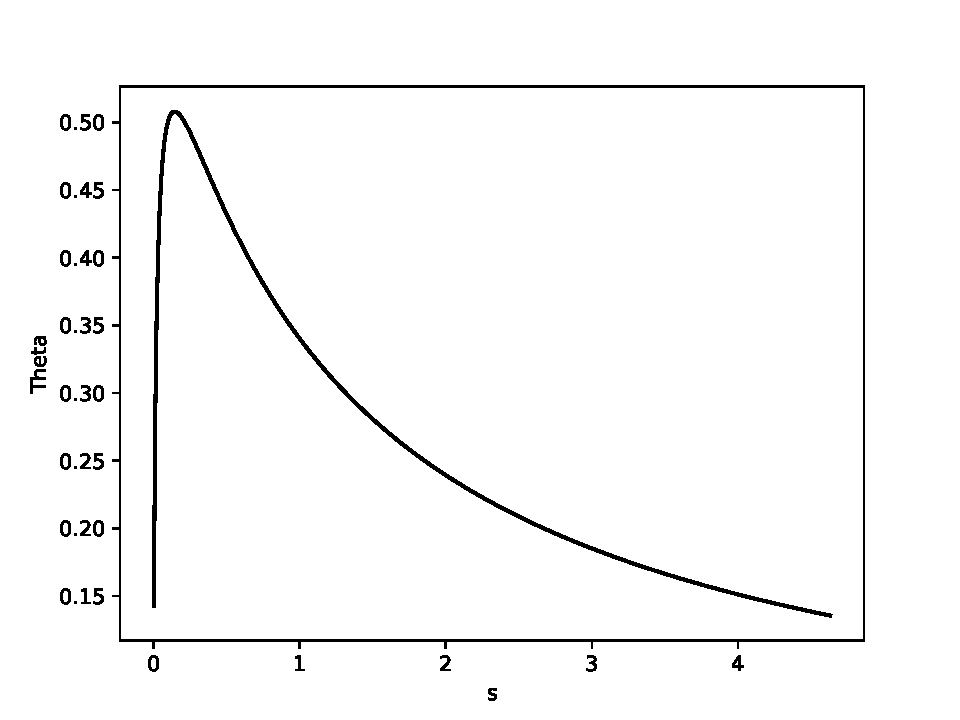
\includegraphics[scale=0.70]{Theta.pdf}
        \caption{偏转角$\Theta$与瞄准距离$s$之间的关系图}
    \end{figure}
    \\
    微分散射截面的公式为:
    \begin{align}
        \sigma(\Theta) = \frac{s}{\sin \Theta}\left|\frac{\d s}{\d \Theta}\right|
    \end{align}
    由于上一步作图时已经得到了比较精确的$\Theta$与$s$的关系,考虑直接使用差分计算微分散射截面,
    可以得到关系图:
    \\
    \begin{figure}[htbp]
        \centering
        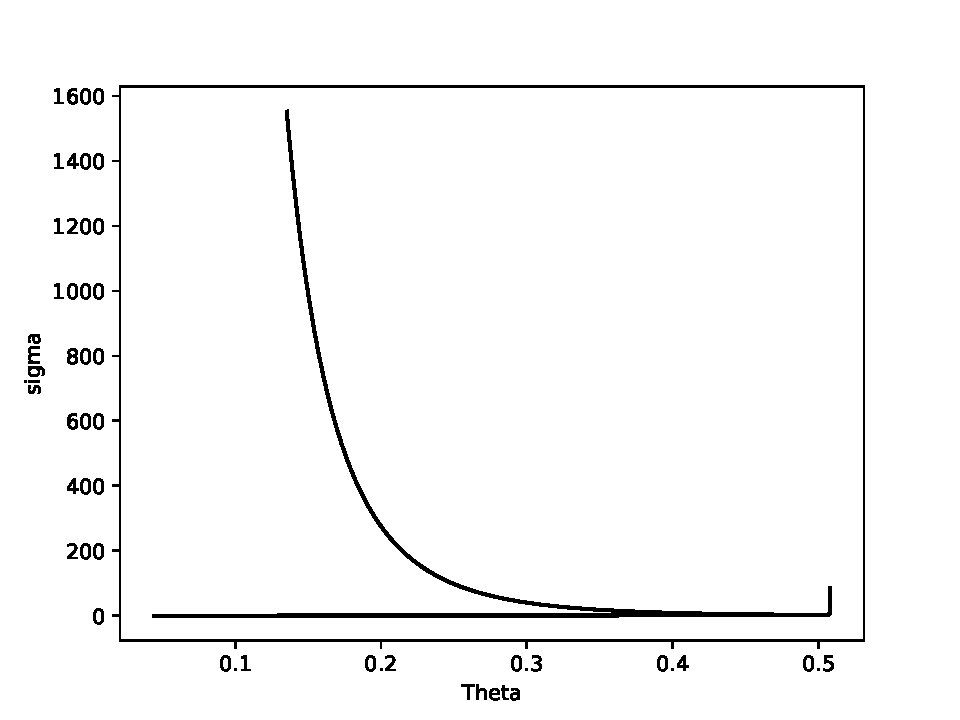
\includegraphics[scale=0.70]{differential.pdf}
        \caption{微分散射截面$\sigma$与偏转角$\Theta$之间的关系图}
    \end{figure}
    \\
    可以从关系图中看出,由于$s$与$\Theta$并不是一一对应的关系,因此图像为一多值函数;由于此散射问题
    存在最大偏转角,因此在最大偏转角处散射截面是发散的,可以在图中看到一个小的尖峰,由于发散地非常快
    ,也没有能很形象地展示处来。
    \\
    \paragraph{第四题\;\;汤川势}
    \begin{align}
        U(r) = -\alpha\frac{\mathrm{e}^{-r/a}}{r}
    \end{align}
    \subparagraph{(a)}汤川势下的运动方程
    \subparagraph{解:}直接套用有心力场中的运动方程:
    \begin{align}
        \frac{\d r}{\d t} &= \sqrt{\frac{2}{m}\left(E + \alpha\frac{\e ^{-r/a}}{r}\right)-\frac{J^{2}}{m^{2}r^{2}}}\\
        \frac{\d \phi}{\d t} &= \frac{J}{mr^{2}}
    \end{align}
    \subparagraph{(b)}有效势能的讨论
    \subparagraph{解:}
    直接给出有效势能的表达式:
    \begin{align}
        U_{eff} = \frac{J^{2}}{2mr^{2}} - \alpha\frac{\mathrm{e}^{-r/a}}{r}
    \end{align}
    首先分析一下有效势能的特征,当$r\to 0$时,汤川势以$r^{-1}$趋近于无穷,所以有效势能总体趋于正无穷;
    当$r\to+\infty$时,汤川势以比指数衰减还要快的速度趋于零,有效势能总体趋于零。因此在这两种情况之间
    ,有可能会出现极值点或者没有极值点。
    考虑有效势能稳定点是否在$r>0$有解,对有效势能求导并令导数等于零:
    \begin{align}
        \frac{J^{2}}{m} = \alpha r(\frac{r}{a} + 1)\e ^{-r/a}
    \end{align}
    那么可以看出当$J$很大时,由于等式右边存在极大值,可能会出现无解的情况,对应于有效势能曲线没有极值点,
    也就是粒子的运动一定是无界的,在时间趋于无穷的情况下粒子一定会运动到势能中心的无穷远处(角动量很大一定意味着能量很大)。
    如果当角动量小到一定程度,上述方程可能会有一个解或者两个解,如果有一个解应对应于极小值,只要粒子的总能量不要高过极小值附近的
    势垒,就可以在有效势能极小值附近作有界运动。当有两个解时,除了一个极小值点,还有一个极大值点,粒子在有效势能极大值点附近的运动是不稳定的,可能会
    掉入能量更低的势阱或者演化成无界运动。
    \subparagraph{(c)}近似圆轨道的近心点进动
    \subparagraph{解:}
    考虑对圆轨道进行一个微扰,讨论微扰后的径向运动和角向运动周期的比值就可以得知近心点处的进动情况,
    理应假设扰动足够小,不足以影响角向运动的周期(依然用圆轨道的周期来计算)。如果扰动后的运动稳定,那么一定是
    在有效势能极小值附近的扰动,此时:
    \begin{align}
        \frac{\d U_{eff}}{\d r}(\rho) &= \alpha\frac{(1 + \rho/a)}{\rho^{2}}\e ^{-\rho/a} - \frac{J^{2}}{m\rho^{3}} = 0\\
        \frac{J^{2}}{m} &=  \alpha \rho(\rho/a + 1)\e ^{-\rho/a}
    \end{align}
    其中$\rho$为圆轨道半径,此时我们考虑扰动为$r(t) = \rho + \eta(t)$,认为扰动前后角动量和能量都可以近似看作不变,
    写出扰动前后的能量守恒表达式:
    \begin{align}
        E &= \frac{J^{2}}{2m\rho^{2}} - \alpha\frac{\e^{-\rho/a}}{\rho}\\
        E &= \frac{1}{2}m\dot{\eta}^{2} + \frac{J^{2}}{2m(\rho + \eta)^{2}} - \alpha\frac{\e^{-(\rho + \eta)/a}}{\rho + \eta}
    \end{align}
    将第二式展开到$\eta$的二阶,然后带入圆轨道条件与圆轨道上的能量表达式,化简后零阶项与一阶项均被消掉:
    \begin{align}
        0 = \frac{1}{2}m\dot{\eta}^{2} + \frac{\alpha}{\rho}\e ^{-\frac{\rho}{a}}\frac{a\rho + a^{2} - \rho^{2}}{2a^{2}\rho^{2}}\eta^{2}
    \end{align}
    上式两边求导后可得一标准的简谐振动方程,振动的角频率,即径向运动的角频率为:
    \begin{align}
        \delta\omega = \sqrt{\frac{\alpha}{m\rho}\e ^{-\frac{\rho}{a}}\frac{a\rho + a^{2} - \rho^{2}}{a^{2}\rho^{2}}}
    \end{align}
    容易得到在微扰前圆轨道上的运动的角频率,即角向运动的角频率为:
    \begin{align}
        \omega = \sqrt{\frac{\alpha}{m\rho}\e ^{-\frac{\rho}{a}}\frac{a\rho + a^{2}}{a^{2}\rho^{2}}}
    \end{align}
    何为近心点进动的角度?径向运动达到一个周期之后,角向运动比$2\pi$多出的角度就是近心点进动的角度:
    \begin{align}
        \Delta\phi &= \frac{2\pi\omega}{\delta\omega} - 2\pi = 2\pi\left(\sqrt{\frac{\rho + a}{\rho + a - \rho^{2}/a}} - 1\right)
    \end{align}
    如果考虑$a$很大,那么进动角度可以近似:
    \begin{align}
        \Delta\phi = 2\pi\left(\frac{1}{\sqrt{1 - \frac{\rho^{2}}{a^{2}}}} - 1\right) = \pi\frac{\rho^{2}}{a^{2}}
    \end{align}
    \subparagraph{(d)}汤川势的散射
    \subparagraph{解:}
    考虑$a$非常大时的情形,此时势能可以展开为:
    \begin{align}
        U(r) = -\alpha\frac{\e ^{-\frac{r}{a}}}{r} = -\alpha\frac{1}{r}(1-\frac{r}{a}) = -\frac{\alpha}{r} + \frac{\alpha}{a}
    \end{align}
    首先给出偏转角的积分表达式:
    \begin{align}
        \varphi = 2s\int_{r_{0}}^{+\infty}\frac{1/r^{2}\d r}{\sqrt{(1 - U(r)/E) - b^{2}/r^{2}}}
    \end{align}
    d带入此题中的势能表达式:
    \begin{align}
        \varphi = 2s\int_{r_{0}}^{+\infty}\frac{1/r^{2}\d r}{\sqrt{\left(1 - \frac{\alpha}{aE}\right) + \frac{\alpha}{rE} - \frac{b^{2}}{r^{2}}}}
    \end{align}
    其中$r_{0}$为近心点到散射中心的距离,同时也是上式被积函数分母的零点,将分母配方并换元可以得到(此时用到了
    $r_{0}$是分母零点的这个事实):
    \begin{align}
        \varphi = \arccos\frac{\frac{\alpha}{2sE}}{\sqrt{1-\frac{\alpha}{aE} + \frac{\alpha^{2}}{4s^{2}E^{2}}}}
    \end{align}
    化简一下:
    \begin{align}
        \cos^{2}\varphi = \frac{\frac{\alpha^{2}}{4s^{2}E^{2}}}{1-\frac{\alpha}{aE} + \frac{\alpha^{2}}{4s^{2}E^{2}}}
    \end{align}
    再根据$\Theta = \pi - 2\varphi$,我们得到了瞄准距离和偏转角之间的关系:
    \begin{align}
        s^{2} = \frac{\alpha^{2}}{4E^{2}\left(1 - \frac{\alpha}{aE}\right)}\cot^{2}\frac{\Theta}{2}
    \end{align}
    带入微分散射截面的公式:
    \begin{align}
        \frac{\d \sigma}{\d\Omega} = -\frac{s\d s}{\sin\Theta \d \Theta} = \frac{1}{4}\frac{\alpha^{2}}{m^{2}v_{\infty}^{4}\left(1 - \frac{2\alpha}{amv_{\infty}^{2}}\right)}\csc^{4}\frac{\Theta}{2}
    \end{align}
    \paragraph{第五题}
    \subparagraph{(a)解:}
    令两个物体的位置分别为$x_{1},\;x_{2}$,选取平衡位置为零点,容易写出系统的拉格朗日量:
    \begin{align}
        L = \frac{1}{2}m(\dot{x_{1}}^{2} + \dot{x_{2}}^{2}) - \frac{1}{2}kx_{1}^{2} - \frac{3}{2}k(x_{1} - x_{2})^{2} - \frac{1}{2}kx_{2}^{2}
    \end{align}
    \begin{gather}
    (m_{ij}) = 
        \begin{bmatrix}
            m & 0\\
            0 & m
        \end{bmatrix}
        \quad
    (k_{ij}) = 
        \begin{bmatrix}
            4k & -3k\\
            -3k & 4k
        \end{bmatrix}
    \end{gather}
    容易写出久期行列式:
    \begin{gather}
    \begin{vmatrix}
        m\omega^{2} - 4k & 3k\\
        3k & m\omega^{2} - 4k
    \end{vmatrix}
    =0
    \end{gather}
    解得特征频率为$\omega_{1} = \sqrt{\frac{k}{m}},\;\omega_{2} = \sqrt{\frac{7k}{m}}$。
    \subparagraph{(b)解:}
    考虑考虑库仑相互作用后体系的平衡位置会发生变化,两个物块偏离上一问平衡位置的距离(偏离弹簧原厂的距离)为$\Delta x$,
    考虑使用新的平衡位置为零点,写出体系的拉格朗日量:
    \begin{align}
        L &= \frac{1}{2}m(\dot{x_{1}}^{2} + \dot{x_{2}}^{2}) - \frac{1}{2}k(x_{1} - \Delta x)^{2} - \frac{1}{2}k(x_{1} - x_{2} + 2\Delta x)^{2} - \frac{1}{2}k(x_{2} + \Delta x)^{2} - \frac{1}{4\pi\epsilon_{0}}\cdot\left(\frac{q^{2}}{l + x_{2} - x_{1}} - \frac{1}{l}\right)\\
        l &= l_{0} + 2\Delta x
    \end{align}
    考虑小振动的条件,将库伦作用按$(x_{2} - x_{1})$展开,由于选取了平衡位置为势能零点,展开后的一次项相互消去,同时我们忽略掉常数项,拉格朗日量可以近似为:
    \begin{align}
        L = \frac{1}{2}m(\dot{x_{1}}^{2} + \dot{x_{2}}^{2}) - \frac{1}{2}kx_{1}^{2} - \frac{1}{2}k(x_{1} - x_{2})^{2} - \frac{1}{2}kx_{2}^{2} - \frac{q^{2}}{4\pi\epsilon_{0}l^{3}}(x_{2} - x_{1})^{2}
    \end{align}
    记$\frac{q^{2}}{2\pi\epsilon_{0}l^{3}} = k'$,得到:
    \begin{gather}
        (m_{ij}) = 
            \begin{bmatrix}
                m & 0\\
                0 & m
            \end{bmatrix}
            \quad
        (k_{ij}) = 
            \begin{bmatrix}
                2k + k' & -k - k'\\
                -k - k' & 2k + k'
            \end{bmatrix}
    \end{gather}
    得到久期行列式为:
    \begin{gather}
        \begin{vmatrix}
            m\omega^{2} - 2k - k' & k + k'\\
            k + k' & m\omega^{2} - 2k - k'
        \end{vmatrix}
        =0
    \end{gather}
    容易得到$\omega_{1} = \sqrt{\frac{k}{m}},\;\omega_{2} = \sqrt{\frac{3k + 2k'}{m}}$,其中$k'$已经有过定义,
    平衡后两物体之间的距离可以通过库仑定律算出,可以由下式给出:
    \begin{align}
        3k\Delta x = \frac{q^{2}}{4\pi\epsilon_{0}}\cdot\frac{1}{(l_{0}^{2} + 2 \Delta x )^{2}}
    \end{align}
    \paragraph{第六题\;\;分子振动}
    \subparagraph{解:}
    三个原子的质量分别为$m,\;M,\;m$,假设在$x$方向上的弹簧劲度系数为$k$,由于三个自由度没有耦合,可以
    分别讨论(写成整体的矩阵也一定是分块对角的),$x$方向的势能也可以写成题目中类似的形式,我们只讨论一个
    方向就行,考虑$x$方向:
    \begin{align}
        L = \frac{1}{2}m\dot{x_{1}}^{2} + \frac{1}{2}M\dot{x_{2}}^{2} + \frac{1}{2}m\dot{x_{3}}^{2} - \frac{k}{2}(x_{2} - x_{1})^{2} - \frac{k}{2}(x_{3} - x_{2})^{2}
    \end{align}
    \begin{gather}
        (m_{ij}) = 
            \begin{bmatrix}
                m & 0 & 0\\
                0 & M & 0 \\
                0 & 0 & m
            \end{bmatrix}
            \quad
        (k_{ij}) = 
            \begin{bmatrix}
                k & -k & 0\\
                -k & 2k & -k\\
                0 & -k & k
            \end{bmatrix}
    \end{gather}
    得到久期行列式为:
    \begin{gather}
        \begin{vmatrix}
            m\omega^{2} - k & k &0\\
            k & M\omega^{2} - 2k & k\\
            0 & k & m\omega^{2} - k
        \end{vmatrix}
        =0
    \end{gather}
    可以解得三个特征频率为$\omega_{1} = 0,\;\omega_{2} = \sqrt{\frac{(2m + M)k}{Mm}},\;\omega_{3} = \sqrt{\frac{k}{m}}$。
    我们可以解出模态矩阵:
    \begin{gather}
        A = 
        \begin{bmatrix}
            \frac{1}{\sqrt{2m + M}} & \frac{1}{\sqrt{2m}} & \frac{\sqrt{M}}{2m}\\
            \frac{1}{\sqrt{2m + M}} & 0 & -\frac{1}{\sqrt{M}}\\
            \frac{1}{\sqrt{2m + M}} & -\frac{1}{\sqrt{2m}} & \frac{\sqrt{M}}{2m}
        \end{bmatrix}
    \end{gather}
    那么简正坐标可以表示为:
    \begin{align}
        Q = A^{-1}x = (A^{t}(m_{ij}))x
    \end{align}
    这样就能从简正坐标的形式上看出(由于质量矩阵有着对角的形式,这比较容易看),零频振动是由于分子整体平动引起的(每个原子都向同一个方向同步移动);
    $\omega_{3} = \sqrt{\frac{k}{m}}$这个振动是由于两侧原子相对运动(中心原子不动)产生的;
    $\omega_{2} = \sqrt{\frac{(2m + M)k}{Mm}}$是两侧原子同向运动,中心原子反向运动产生的振动。
    \par
    对于另外两个方向,讨论完全类似,可以得到几乎相同的结果。
    \\
    \paragraph{第七题}
    \subparagraph{解:}
    虽然这是一道理论力学题目,但是为了方便计算弹簧伸长量,我还是选择了进行受力分析,考虑平衡时的受力情况,设
    弹簧上的拉力为$T$,可以得到:
    \begin{align}
        2T\cos\theta_{0} = mg\\
        k\Delta x = T
    \end{align}
    那么弹簧的伸长量为:
    \begin{align}
    \Delta x = \frac{mg}{2k\cos\theta_{0}}
    \end{align}
    将弹簧平衡时的长度记为:
    \begin{align}
        a = b + \Delta x = b + \frac{mg}{2k\cos\theta_{0}}
    \end{align}
    这个在平面上运动的刚体一共有3个自由度,选取刚体的质心坐标$(x, y)$与刚体轴线与平衡时轴线的夹角$\phi$为广义坐标,
    选取逆时针的那个小的转角为正,首先很容易给出刚体的动能:
    \begin{align}
        T = \frac{1}{2}m(\dot{x}^{2} + \dot{y}^{2}) + \frac{1}{12}ml^{2}\dot{\phi}^{2}
    \end{align}
    选取平衡时的刚体质心为坐标原点,那么可以给出弹簧的左右固定悬挂点坐标:
    \begin{align}
        \left(-\frac{l}{2} - a\sin\theta_{0},\; a\cos\theta_{0}\right)\\
        \left(\frac{l}{2} + a\sin\theta_{0},\; a\cos\theta_{0}\right)
    \end{align}
    一般情况下,刚体左右两端的悬挂点坐标为:
    \begin{align}
        \left(x - \frac{l}{2}\cos\phi,\;y - \frac{l}{2}\sin\phi\right)\\
        \left(x + \frac{l}{2}\cos\phi,\;y + \frac{l}{2}\sin\phi\right)
    \end{align}
    那么可以算出两个弹簧一般情况下的长度:
    \begin{align}
        l_{1} &= \sqrt{\left(\frac{l}{2} + a\sin\theta_{0} + x - \frac{l}{2}\cos\phi\right)^{2} + \left(a\cos\theta_{0} - y + \frac{l}{2}\sin\phi\right)^{2}}\\
        l_{2} &= \sqrt{\left(\frac{l}{2} + a\sin\theta_{0} - x - \frac{l}{2}\cos\phi\right)^{2} + \left(a\cos\theta_{0} - y - \frac{l}{2}\sin\phi\right)^{2}}
    \end{align}
    弹簧的长度与势能直接相关,我们只用在根号下保留到广义坐标的二次项就行,所以弹簧的长度可以化简为:
    \begin{align}
        l_{1}&= \sqrt{a^{2} + x^{2} + y^{2} + \left(\frac{al\sin\theta_{0}}{2} + \frac{l^{2}}{4}\right)\phi^{2} - ly\phi + 2a(x\sin\theta_{0} - y\cos\theta_{0}) + la\cos\theta_{0}\phi}\\
        l_{2}&= \sqrt{a^{2} + x^{2} + y^{2} + \left(\frac{al\sin\theta_{0}}{2} + \frac{l^{2}}{4}\right)\phi^{2} + ly\phi - 2a(x\sin\theta_{0} + y\cos\theta_{0}) - la\cos\theta_{0}\phi}
    \end{align}
    考虑到质心的重力势能,势能的总和可以写为:
    \begin{align}
        U = mgy + \frac{1}{2}k(l_{1} - b)^{2} + \frac{1}{2}k(l_{2} - b)^{2} - k\Delta x^{2}
    \end{align}
    对势能进行展开,忽略常数项,由于平衡位置是势能的极小值点,所以展开中一次项必定为零,我们不再详细计算,
    重点关注二次项,“不难算出”:
    \begin{align}
        U &= k\left(\sin^{2}\theta_{0} + \frac{mg}{2ak}\cos\theta_{0}\right)x^{2} + k\left(\cos^{2}\theta_{0} + \frac{mg}{2ak\cos\theta_{0}}\sin^{2}\theta_{0}\right)y^{2}\\
        &+ k\left[\frac{l^{2}}{4}\cos^{2}\theta_{0} + \frac{mgl\sin\theta_{0}}{8k\cos\theta_{0}}\left(2 + \frac{l}{a}\sin\theta_{0}\right)\right]\phi^{2} + kl\sin\theta_{0}\left(\cos\theta_{0} - \frac{mg}{2ka}\right)x\phi
    \end{align}
    那么就可以写出系统的拉格朗日量,给出系统的质量矩阵和势能矩阵:
    \begin{gather}
        (m_{ij}) = 
        \begin{bmatrix}
            m & 0 & 0\\
            0 & m & 0\\
            0 & 0 & \frac{1}{6}ml^{2}
        \end{bmatrix}
    \end{gather}
    \begin{gather}
        (k_{ij}) = 
        \begin{bmatrix}
            k\left(2\sin^{2}\theta_{0} + \frac{mg}{ak}\cos\theta_{0}\right) & 0 & kl\sin\theta_{0}\left(2\cos\theta_{0} - \frac{mg}{ka}\right)\\
            0 & k\left(2\cos^{2}\theta_{0} + \frac{mg}{ak\cos\theta_{0}}\sin^{2}\theta_{0}\right) & 0\\
            0 & 0 & k\left[\frac{l^{2}}{2}\cos^{2}\theta_{0} + \frac{mgl\sin\theta_{0}}{4k\cos\theta_{0}}\left(2 + \frac{l}{a}\sin\theta_{0}\right)\right]
        \end{bmatrix}
    \end{gather}
    那么,可以给出系统的久期行列式:
    \begin{gather}
        \begin{vmatrix}
            m\omega^{2} - k\left(2\sin^{2}\theta_{0} + \frac{mg}{ak}\cos\theta_{0}\right) & 0 & - kl\sin\theta_{0}\left(2\cos\theta_{0} - \frac{mg}{ka}\right)\\
            0 & m\omega^{2} - k\left(2\cos^{2}\theta_{0} + \frac{mg}{ak\cos\theta_{0}}\sin^{2}\theta_{0}\right) & 0\\
            0 & 0 & \frac{1}{6}ml^{2}\omega^{2} - k\left[\frac{l^{2}}{2}\cos^{2}\theta_{0} + \frac{mgl\sin\theta_{0}}{4k\cos\theta_{0}}\left(2 + \frac{l}{a}\sin\theta_{0}\right)\right]
        \end{vmatrix}
        \\
        = 0
    \end{gather}
    (太宽了,凑活一下)可以给出系统的特征频率:
    \begin{align}
        \omega_{1} &= \sqrt{\frac{k}{m}\left(2\sin^{2}\theta_{0} + \frac{mg}{ak}\cos\theta_{0}\right)}\\
        \omega_{2} &= \sqrt{\frac{k}{m}\left(2\cos^{2}\theta_{0} + \frac{mg}{ak\cos\theta_{0}}\sin^{2}\theta_{0}\right)}\\
        \omega_{3} &= \sqrt{\frac{6k}{ml^{2}}\left[\frac{l^{2}}{2}\cos^{2}\theta_{0} + \frac{mgl\sin\theta_{0}}{4k\cos\theta_{0}}\left(2 + \frac{l}{a}\sin\theta_{0}\right)\right]}
    \end{align}
    其中$a$是弹簧处于平衡位置时的长度,与原长$b$的关系之前已经给出(我算不出来简正模了……)。
    \paragraph{第八题\;\;圆管中滚动的圆柱体}
    \subparagraph{(a)解:}
    容易直接给出题目中要求的关系(注意到这里的关系并没有用到圆柱在圆管中纯滚的条件,感觉只有在计算转动动能时这一条件才会起作用):
    \begin{align}
        X(t) &= R\cdot\theta(t)\\
        x(t) &= X(t) + \frac{R}{2}\sin\phi(t)\\
        y(t) &= R - \frac{R}{2}\cos\phi(t)
    \end{align}
    \subparagraph{(b)解:}
    \begin{align}
        \dot{X} &= R\dot{\theta}\\
        \dot{x} &= R\dot{\theta} + \frac{R}{2}\dot{\phi}\cos\phi\\
        \dot{y} &= \frac{R}{2}\dot{\phi}\sin{\phi}
    \end{align}
    \subparagraph{(c)解:}
    平动动能可以直接由$\dot{X}$给出:
    \begin{align}
        T_{M,t} = \frac{1}{2}M\dot{X}^{2} = \frac{1}{2}MR^{2}\dot{\theta}^{2}
    \end{align}
    转动动能可以直接由$\dot{\theta}$给出:
    \begin{align}
        T_{M,r} = \frac{1}{2}I\omega^{2} = \frac{1}{2}MR^{2}\dot{\theta}^{2}
    \end{align}
    平动动能和转动动能大小一致。
    \subparagraph{(d)解:}
    圆柱体的平动动能可以方便地用圆柱体的质心坐标$(x,\;y)$来表示:
    \begin{align}
        T_{m,t} = \frac{1}{2}m(\dot{x}^{2} + \dot{y}^{2})
    \end{align}
    带入(b)中结论:
    \begin{align}
        T_{m,t} = \frac{1}{2}mR^{2}\left(\dot{\theta}^{2} + \dot{\theta}\dot{\phi}\cos\phi + \frac{\dot{\phi}^{2}}{4}\right)
    \end{align}
    \subparagraph{(e)解:}
    关键是圆柱运动的角速度怎么求,可以肯定的是圆柱的角速度一定可以写成$\dot{\theta},\;\dot{\phi}$的线性组合,只需要考虑两种特殊的情况
    就可以确定系数,那么分别考虑$\dot{\theta}=0,\;\dot{\phi}=0$可以得到: 
    \begin{align}
        \omega_{m} = 2\dot{\theta} + \dot{\phi}
    \end{align}
    那么容易写出圆柱转动动能:
    \begin{align}
        T_{m,r} &= \frac{1}{2}I_{m}\omega_{m}^{2} = \frac{mR^{2}}{16}(2\dot{\theta} + \dot{\phi})^{2}\\
        &= \frac{mR^{2}}{16}(4\dot{\theta}^{2} + 4\dot{\theta}\dot{\phi} + \dot{\phi}^{2})
    \end{align}
    \subparagraph{(f)解:}
    体系的重力势能比较容易写出,由于圆筒的质心高度不变,我们选取圆筒的质心$Y$坐标为零势能面,只有圆柱对重力势能有贡献
    那么体系的重力势能可以表达为:
    \begin{align}
        U = mg(y - R) = -\frac{R}{2}mg\cos\phi
    \end{align}
    那么拉格朗日量为:
    \begin{align}
        L &= T - U = T_{M,t} + T_{M,r} + T_{m,t} + T_{m,r} - U\\
        & = R^{2}\left(M + \frac{3}{4}m\right)\dot{\theta}^{2} + \frac{mR^{2}}{4}(1 + 2\cos\phi)\dot{\phi}\dot{\theta} + \frac{3}{16}mR^{2}\dot{\phi}^{2} + \frac{R}{2}mg\cos\phi
    \end{align}
    \subparagraph{(g)解:}
    体系的运动方程可以直接由拉格朗日方程求出:
    \begin{align}
        \frac{\d}{\d t} \frac{\partial L}{\partial \dot{q}} - \frac{\partial L}{\partial q} = 0
    \end{align}
    带入(f)中算出的拉格朗日量,得到体系的运动方程:
    \begin{align}
        2(4M + 3m)\dot{\theta} + m(1 + 2\cos\phi)\dot{\phi} = C_{0}\\
        2mR(1 + 2\cos\phi)\ddot{\theta} + 3mR\ddot{\phi} + 4mg\sin\phi = 0
    \end{align}
    由于$\theta$为循环坐标,$C_{0}$为一运动积分。
    \subparagraph{(h)解:}
    考虑利用小振动的条件化简一下运动方程,将$\phi\ll1$的条件带入(g)中的第一个运动方程:
    \begin{align}
        2(4M + 3m)\ddot{\theta} + 3m\ddot{\phi} = 0
    \end{align}
    将小振动的条件带入第二个运动方程:
    \begin{align}
        6\ddot{\theta} + 3\ddot{\phi} + \frac{4g}{R}\phi = 0
    \end{align}
    将化简后的第一个运动方程带入化简后的第二个运动方程:
    \begin{align}
        \ddot{\phi} + \frac{4M + 3m}{3M}\frac{g}{R}\phi = 0
    \end{align}
    可以看出体系振动的角频率为$\omega = \sqrt{\frac{4M + 3m}{3M}\frac{g}{R}}$。
\end{document}